%!TEX root=../../thesis_rui_almeida.tex



\section{Tomosim}%
\label{sec:tomosim}

Tomosim was the (somewhat unoriginal) name given to the tomographic
simulation software tool that was designed and built as part of this
project. It was created to tackle the trajectory-related hypothesis,
briefly described in this chapter's introduction.

The final system must be able to gather projection information by
reading spectral information, in this case the \gls{DOAS}-retrieved
column density for an atmospheric trace gas (or several) from a set of
predetermined directions. In "normal" tomographic \gls{DOAS}
application, these directions are fixed and depend on the experiment
infrastructure's geometry (see Section~\ref{sec:doas_tomography}). One
of the main novelties that I am trying to create with this project is a
very high degree of geometric freedom. A mobile system has no custom
infrastructure, and therefore has no fixed positions to which it is
tied. Instead its ability measure and monitor its atmospheric
surroundings relies on its movement. 

A ground-based mobile \gls{DOAS}-tomography system would have too strong
a dependency on open spaces and the topography of its \gls{ROI} to be
useful in any \textit{real world} scenario. A much more interesting and
feasible approach would be to use some kind of flying machine that could
carry spectroscopic equipment, and that could be programmed to fly in a
precise manner. Fortunately, current day technology provides a very
strong immediate candidate: a \gls{UAV} of the n-copter type, such as
the one in Figure~\ref{fig:an_hexacopter}\todo{image citation}.

\begin{figure}[htpb]
    \centering
    \missingfigure{An image of an hexacopter in flight.}
    \caption{Hexacopter in flight. Taken from laksjdlaksjd}
    \label{fig:an_hexacopter}
\end{figure}

A natural choice as it may seem as means for the measurements I am
describing in this document, its programming is almost  as important as
the hardware itself (if not more). The vehicle must be programmed to
describe a very precise (taking into account the type of operation we
are proposing) trajectory. In flight, the drone should be able to carry
and point an optical system towards any direction and in a short time.
Said optical system should be attached to a computer-controlled
spectrometer. This would allow the whole system to determine target
trace gas concentration on demand and programmatically.

The programmed trajectory should make use of these capabilities and
gather enough information for tomographic reconstruction. This also
means that the trajectory must be comprised of a sufficient number of
spectral projection acquisition \emph{opportunities}.

Of the several geometries that are described in the literature for
tomographic reconstructions, the one that seemed to be more promising in
terms of the balance between reconstruction complexity and the
information / flight time ratio was the fanbeam assembly (described in
Section~\ref{sec:tomographic_algorithms_and_reconstruction_techniques}).
It was the feasibility of this trajectory for the proposed purposes that
this simulation aimed to prove.

In essence, the drone's trajectory (illustrated in
Figure~\ref{fig:illustriated_trajectory_and_fanbeam_formation}) is a
horizontal circle which is parametrised to be at a certain height and to
have a certain diameter.  Both of these dimensions are set at experiment
/ measurement time. The drone stops on this circle at regular angular
intervals, say $\alpha$ degrees. Each one of these stops (360 / $\alpha$
stops) will generate a fanbeam projection, by pointing the optical
system inwards (with respect to the circular macro-trajectory) and
performing a series of spectroscopic measurements in different
directions and also at regular intervals, say $\gamma$ degrees. The
particular case in which $\alpha = \gamma$ is very interesting, because
it then opens the possibility for resorting the fanbeams into parallel
virtual-projections that are much easier to reconstruct tomographically,
as introduced in
Section~\ref{sec:tomographic_algorithms_and_reconstruction_techniques}.  

\begin{figure}[htpb]
    \centering
    \missingfigure{}
    \caption{Illustration of the projection gathering algorithm based on
    fanbeam assembly of information. On the left the circle which
    constitutes the general trajectory of the drone. On the right the
    gymbal points the optical system towards different directions, forming
    what can be seen as a fan.}
    \label{fig:illustrated_trajectory_and_fanbeam_formation}
\end{figure}

\subsection{Discretisation}%
\label{sub:discretisation}

Discretisation is the process by which the \gls{ROI} is digitised into a
computational platform. There are several algorithms designed for this
effect that are available in the literature. One of the easiest to
implement that is also adequate to this application (unsurprisingly)
comes from the medical imaging field. It was published in 1985 by Robert
Siddon~\cite{Siddon1985}.

The Siddon algorithm is one of the foremost path calculation algorithms
in the medical field of radiology. It is not only used for the
discretisation of tomographic fields, but also in the dose calculation
process of radiation therapy patients. The idea behind the algorithm is
that the total dose of a radiation ray, i.e., its path, is given by the
sum of the length within each pixel that this ray traverses multiplied
by the density of said pixel~\todo{Ugly. Rewrite}. In mathematical
notation, one can write this as in Equation~\ref{eq:siddon_sum}.

\begin{equation}
    \label{eq:siddon_sum}
    d = \sum_{i}\sum_{j}\sum{k} l(i, j, k)\cdot\rho(i, j, k)
\end{equation}

In Equation~\ref{eq:siddon_sum}, $d$ is the radiological path (the
projection value), $i$, $j$, $k$ are the coordinate vectors, $l$ is the
length within a pixel and $\rho$ is the pixel density. In our case, this
last value is the trace gas column density for that pixel.

The main reason for Siddon's algorithm being easy to implement is its
treatment of pixels (or voxels if in 3D). Instead of considering pixels
as \emph{atomic}\footnote{In their undivisible sense.} units, it defines
them as the intersections of orthogonal sets of equally spaced lines
(planes in 3D). Pixel lengths are determined by the looking at the
intersections between the orthogonal lines and the radiation ray. 

\begin{figure}[htpb]
    \centering
    \missingfigure{Siddon article grid and pixel definition}
    \caption{Grid and pixel definition, as they appear in the original
        article by Robert Siddon~\cite{Siddon1985}. Notice that pixels are formed by line
        intersections.}
    \label{fig:siddon_pixels}
\end{figure}

Since lines are orthogonal and equally spaced, all intersections can be
calculated recursively after knowing where the first intersection is
located. The calculation of the radiologic path is achieved by
determining the subset of the intersections between the orthogonal lines
and the lih+ght ray that identifies individual pixels.

If $P_1 \to (X_1, Y_1)$ and $P_2 \to (X_2, Y_2)$ are the start and
end of the radiologic path within the \gls{ROI}, the line between them
can be parametrically written as in Equation~\ref{eq:p1p2parametric}.

\begin{equation}
\label{eq:p1p2parametric}
    \begin{aligned}
        X(\alpha) = &X_1{} + \alpha \cdot (X_2 - X_1)\\
        Y(\alpha) = &Y_1{} + \alpha \cdot (Y_2 - Y_1)
    \end{aligned}
\end{equation}

In Equation~\ref{eq:p1p2parametric}, $\alpha$ is 0 at $P_1$ and 1 at
point $P_2$. Values of $\alpha$ within the \gls{ROI} vary according to
the positions of $P_1$ and $P_2$ with respect to the \gls{ROI}. By
determining $\alpha$ values of each intersection (in both directions),
one can determine the length of the ray within the pixel by the
difference of adjacent intersections. The whole algorithm can be written
as in Algorithm~\ref{alg:siddon}.

\begin{algorithm}[H]
\SetAlgoLined
\KwResult{Discretised ROI space.}
calculate range of parametric values\;
calculate range of pixel indices\;
calculate parametric sets\;
merge sets\;
calculate pixel(or voxel) lengths\;
calculate pixel indices\;
\caption{Siddon's algorithm's procedural steps. After running this
algorithm, one is able to represent any continuous ray through the
analysis field as a sum of discrete lengths}
\label{alg:siddon}
\end{algorithm}

\subsection{Phantoms}%
\label{sub:phantoms}

A phantom is a device that represents the human body or some of its
parts. They have been used in medical physics since the beginning of the
field. In medical imaging, for instance, phantoms started being used in
the late nineteenth century and early twentieth century. At the time, it
was very difficult to find volunteers for any kind of experiment that
involved radiation, due to the common effects that were rapidly reported
by the first people subject to this kind of
intervention~\cite{Dewerd2014}. In spite of this difficulty, scientists
and researchers still had to determine the dosimetry properties and
physical limitations of their radiative devices, so medical physicists
had to develop their own test models, or phantoms, for this effect. More
recently, phantoms have been designed to develop computed tomography
applications and algorithms. These phantoms mimic the body's attenuation
properties in the X-Ray section of the electromagnetic spectrum, for
instance.

Although the system that I propose does not aim at measuring or using
the human body (or any other animal's), the concept still stands. To
evaluate our reconstruction methods and the validity of our data
gathering strategies, I needed an atmospheric phantom.

The distribution of gases in the atmosphere is completely different from
biological tissue. Therefore, medical imaging phantoms were not
adequate. The design that I have created is based on the premise that a
two-dimensional Gaussian peak is more appropriate to describe the
smoother nature of gaseous distribution~\cite{Stachniss2009}. This in
contrast with the crisply defined edges of a medical tomography phantom
such as Shepp-Logan's head phantom~\cite{Shepp1974}.

To design the phantom itself, I used a library called
TomoPhantom~\cite{Kazantsev2018}, a tomographic phantom generator that
provides a Python \gls{api}, making it trivial to include in the Tomosim
simulator. The new phantom is comprised of 5 Gaussian profiles,
depicting a static gas mixture. An ellipse is also in the phantom, near
one of the corners. This serves mainly as a reference point for
reconstruction, given its more solid and crisp nature. The new phantom
can be seen in Figure~\ref{fig:new_phantom} and its features are stated
in Table~\ref{tab:new_phantom}.


\begin{figure}[htpb]
    \centering
    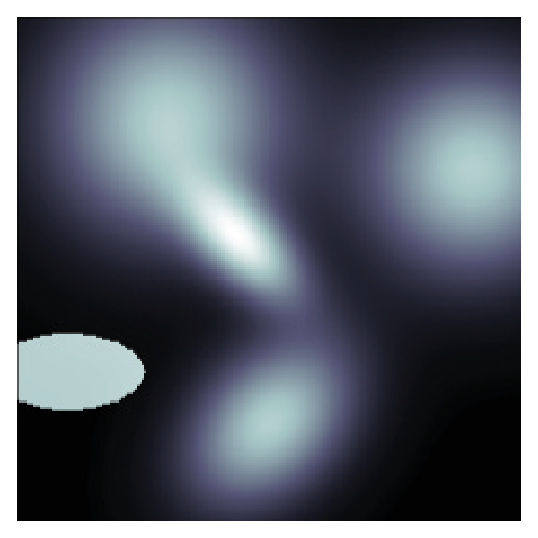
\includegraphics[width=.8\textwidth]{img/eps/original_phantom.eps}
    \caption{A graphical representation of the new spectral phantom,
    custom built for the TomoSim application.}
    \label{fig:new_phantom}
\end{figure}


\begin{table}[htpb]
    \centering
    \caption{Table summarising the new phantom's construction details,
    as a sum of 5 Gaussian profiles and an ellipse designed using
    TomoPhantom. In this table, C0 is the object's amplitude, X0 and Y0
    are its center coordinates, and a and b are the objects half-widths.
    The table is constructed using TomoPhantom's particular syntax and
    more information can be obtained at~\cite{Kazantsev2018}.}
    \label{tab:new_phantom}
    \begin{tabular}{@{}lcccccr@{}}
    \hline
    \textbf{Type} & \textbf{C0} & \textbf{X0} & \textbf{Y0} & \textbf{a}
                  & \textbf{b} & \textbf{\textbf{Angle}} \\ \hline
    Gaussian & 1 & -0,1 & -0,1 & 0,25 & 0,5 & -45 \\
    Gaussian & 1 & 0,6 & 0 & 0,65 & 0,45 & -45 \\
    Gaussian & 1 & -0,6 & -0,4 & 0,8 & 0,8 & 0 \\
    Gaussian & 1 & -0,4 & 0,8 & 0,7 & 0,7 & 0 \\
    Ellipse & 1 & 0,4 & -0,8 & 0,3 & 0,15 & 0 \\ \hline
    \end{tabular}
\end{table}

\subsection{Error Estimation}%
\label{sub:error_estimation}

Error sources for the Tomosim simulator come in four different natures:
time errors, geometric errors, spectroscopic errors and reconstruction
errors.

Time errors come from the fact that there are two moments of
measurement. In a dynamic system, the time that passes between the two
is enough for concentrations to change significantly. Tomosim does not
address these errors, because they can be eliminated by the introduction
of a second drone carrying the same type of equipment, which would
eliminate said time difference.

Geometric errors exist due to the drone not being able to situate
itself perfectly. There is always a positioning error, no matter how
sophisticated the onboard equipment is. This type of error is addressed
in the simulation through a Monte Carlo like approach.

Positioning and pointing errors are assumed to have normal
distributions. Each time a point is calculated by the drone, a normally
distributed random number, with a mean if 0 and a standard deviation
equal to the nominal error of the positioning system. This number is
then added to the theoretical point.
Figure~\ref{fig:geometric_error_calculation} is a graphical
representation of the reasoning behind the calculation of the geometric
error. The image deals with two types of error. One comes from the
\gls{rtk} positioning system (the positioning error, $\epsilon_p$); and
the other that comes from the gimbal (the pointing error,
$\epsilon_\gamma$). The two $\epsilon$ values are the nominal error for
the positioning and the pointing devices. The error is introduced in the
simulation through the values of $\beta$ and $D$ (see
Figure~\ref{fig:p2_calculation}) while calculating $P_2$. Given the very
low nominal error for the gimbal, the small angle approximation is valid
($\sin \theta = \theta$). This is used to determine the theoretical
value of $P_2$, located on the device's circular trajectory. Finally,
the software adds the positioning error, using the same process as in
$P_1$'s case. The error depiction in
Figure~\ref{fig:geometric_error_calculation} is extremely exaggerated
for visibility.

\begin{figure}[htpb]
    \centering
    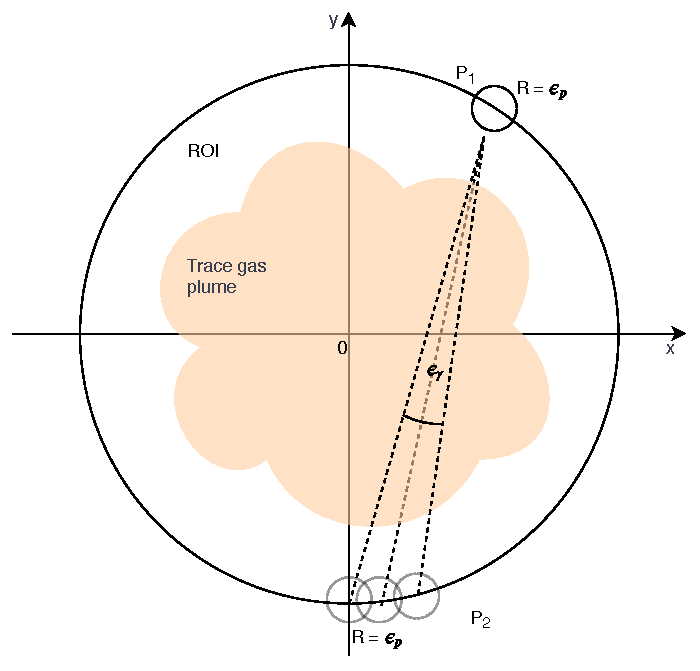
\includegraphics[width=0.8\textwidth]{img/pdf/error_estimation_2.pdf}
    \caption{Error estimation graphical representation. Note errors are
    extremely exaggerated for visualisation purposes.}
    \label{fig:geometric_error_calculation}
\end{figure}

The third type of error are the spectroscopic errors. These come from
the spectroscopic equipment that is used to gather projections. To take
this noise into account, the simulator adds a Gaussian noise spectrum to
each measurement, which is configurable through its standard deviation,
as was previously done in~\cite{Stutz1996}. This is a valid approach,
insofar as the captured spectra are perfectly calibrated regarding
spectral shift and squeeze. Since this is a simulation software, this is
an acceptable assumption.

The final type of error that the system needs to contend with is the
reconstruction error. In tomographic inversion problems, it is common to
use techniques such as the \gls{mse} as a metric for an algorithm's
performance. Tomosim was also evaluated in this light and in two
separate ways. The first was to calculate the \gls{mse} for each pixel of the
whole image. This information can still be viewed as an image (it is a
two-dimensional grid of values) and paints an immediate picture of the
general behaviour of the reconstruction algorithm. Moreover, it can tell
the viewer if there are any types of shapes or areas in which the
algorithm has more difficulties. The second way of using \gls{mse} to
evaluate the reconstruction is to calculate a score through
Equation~\ref{eq:mse_score}. In this equation, and with respect to this
simulator, $f$ is the original image and $g$ the one reconstructed from
projections.

\begin{equation}
    \centering
    \label{eq:mse_score}
    E = \sqrt{\frac{\sum\lvert g(x,y) - f(x,y)
    \lvert^{^{2}}}{\sum\lvert f(x,y) \lvert ^{^{2}}}}
\end{equation}
